% CVPR 2025 Paper Template; see https://github.com/cvpr-org/author-kit

\documentclass[10pt,twocolumn,letterpaper]{article}
\usepackage{ctex}
\usepackage{listings}
\usepackage{multirow}
\usepackage[T1]{fontenc}

%%%%%%%%% PAPER TYPE  - PLEASE UPDATE FOR FINAL VERSION
% \usepackage{cvpr}              % To produce the CAMERA-READY version
\usepackage[review]{cvpr}      % To produce the REVIEW version
% \usepackage[pagenumbers]{cvpr} % To force page numbers, e.g. for an arXiv version

% Import additional packages in the preamble file, before hyperref
%
% --- inline annotations
%
\newcommand{\red}[1]{{\color{red}#1}}
\newcommand{\todo}[1]{{\color{red}#1}}
\newcommand{\TODO}[1]{\textbf{\color{red}[TODO: #1]}}
% --- disable by uncommenting  
% \renewcommand{\TODO}[1]{}
% \renewcommand{\todo}[1]{#1}



% It is strongly recommended to use hyperref, especially for the review version.
% hyperref with option pagebackref eases the reviewers' job.
% Please disable hyperref *only* if you encounter grave issues, 
% e.g. with the file validation for the camera-ready version.
%
% If you comment hyperref and then uncomment it, you should delete *.aux before re-running LaTeX.
% (Or just hit 'q' on the first LaTeX run, let it finish, and you should be clear).
\definecolor{cvprblue}{rgb}{0.21,0.49,0.74}
\usepackage[pagebackref,breaklinks,colorlinks,allcolors=cvprblue]{hyperref}

%%%%%%%%% PAPER ID  - PLEASE UPDATE
%\def\paperID{*****} % *** Enter the Paper ID here
\def\paperID{22302010011} % *** Enter the Paper ID here
\def\confName{CVPR}
\def\confYear{2024}

%%%%%%%%% TITLE - PLEASE UPDATE
%\title{\LaTeX\ Author Guidelines for \confName~Proceedings}
\title{Intelligent Document Tampering Detection \confName~Experiment Report}

%%%%%%%%% AUTHORS - PLEASE UPDATE
%\author{First Author\\
%Institution1\\
%Institution1 address\\
%{\tt\small firstauthor@i1.org}
% For a paper whose authors are all at the same institution,
% omit the following lines up until the closing ``}''.
% Additional authors and addresses can be added with ``\and'',
% just like the second author.
% To save space, use either the email address or home page, not both
%\and
%Second Author\\
%Institution2\\
%First line of institution2 address\\
%{\tt\small secondauthor@i2.org}
%}

\author{Team Name\\
{\tt\small 专业课和我作队}
\and
郑光铭\\
{\tt\small 22302010014}
% For a paper whose authors are all at the same institution,
% omit the following lines up until the closing ``}''.
% Additional authors and addresses can be added with ``\and'',
% just like the second author.
% To save space, use either the email address or home page, not both
\and
陈柏滔\\
{\tt\small 22302010008}
\and
黄宸一\\
{\tt\small 22302010011}
}


\begin{document}
\maketitle
\begin{abstract}
    In this experiment, the Faster R-CNN and YOLO models were used as baselines and innovated upon to complete the document tampering detection task. By introducing region threshold filtering, multi-scale data augmentation, and adjusting parameters such as the number of training epochs, batch size, and unified image size, the YOLO11m model was used to achieve the best detection performance, with the highest Micro-F1 score reaching 93.68.
\end{abstract}

\section{Task Introduction}
\label{sec:intro}
%-------------------------------------------------------------------------
\subsection{Task Background}

Verification of vouchers and documents is a perennial topic in financial scenarios and holds extremely important application value in various fields. In particular, the exploration of tampering detection in non-standard documents has always been an important research direction in both industry and academia. With the continuous development of information technology, a large amount of data and information is rapidly flooding into our lives, and the authenticity and reliability of these data and information are crucial. The rapid innovative growth in multimedia technology has made it easily accessible to play with image editing software, which could result in the desired manipulation of the original content. Images are often used as solid evidence in legal proceedings.\cite{SANDHYA2024301663, LiuHaoyue2021RGBN} In the context of digital financial services, the verification of vouchers and documents is even more important. The essence of digital finance is based on the flow and exchange of data and information, and the authenticity and reliability of these data and information are key to whether digital financial services can proceed smoothly. For example, in digital payment scenarios, the authenticity of user payment vouchers directly affects the security and efficiency of payments; in digital lending scenarios, the authenticity of the personal loan information provided by borrowers is the foundation for assessing their repayment ability and risk level. Moreover, the transaction processes and business models in digital finance also raise higher requirements for the verification of vouchers and documents. In digital financial transactions, the verification of vouchers and documents not only needs to ensure their authenticity and reliability, but also needs to guarantee that they are tamper-proof and cannot be forged, to ensure the security and credibility of digital financial transactions. Therefore, the verification of vouchers and documents holds critical application value in digital finance, and developing a set of universal tampering detection algorithms to ensure the authenticity of data collection in various complex scenarios is not only of great business value but also helps reduce various fraud risks, providing a reliable data and information foundation for digital financial services and promoting the stable development of the digital finance industry.

In recent years, deep neural networks (DNNs), such as Convolutional Neural Network (CNN), Recurrent Neural Network (RNN) and Generative Adversarial Networks (GAN) have shown to be capable of characterizing the complex statistical dependencies from high-dimensional sensory inputs and efficiently learning their hierarchical representations, allowing them generalize well across a wide variety of computer vision (CV) tasks, including image forgery detection.\cite{8977568, article}

In this experiment, we will build upon existing detection models and make adjustments and innovations to design an algorithm that identifies tampered regions in voucher images.

\subsection{Task Data}

\subsubsection{Data Format}

The image data used for training and validation can be categorized into shooting documents, receipts, scanned documents/PDFs, and street view photos, etc. The formats of the images include jpg, JPEG, and png, and each image file has a corresponding index.

Some of these images may have been tampered with using common methods such as copy-move, splicing, or removal, as well as more recent deep learning-based image generation techniques.

Tampering localization has also become a research hotspot in image tampering detection tasks in recent years. In practical applications, merely detecting whether an image has been tampered with is not sufficient. It is necessary to also identify where the tampering has occurred in the image.\cite{18512} For simplicity, in this experiment, all tampered regions are assumed to be rectangular.

The label file stores the tampered region (which may be empty) corresponding to each image file, and the specific format is as follows:
\begin{quote}
  [\dots

  \{``id'': ``fileName'', ``region'': [$[x_1, y_1, x_2, y_2]$]\},

  \dots,

  \{``id'': ``fileName2'', ``region'': []\},

  \dots]
\end{quote}

fileName refers to the corresponding image file name. If the image is tampered with, the region is $[x_1, y_1, x_2, y_2]$, representing the pixel coordinates of the top-left and bottom-right corners of the rectangular tampered area. If not tampered with, the region is empty.

\subsubsection{Data Split}

The images in the above format are divided into a training set and a test set, with the respective quantities of 13,000 images and 5,000 images.

The training set has a corresponding label file `label\_train.json' for training, which stores the tampered regions (which may be empty) for each image in the training set. The filenames in the training set are all in the format `train\_$index$', such as `train\_8359.jpg'.

For the YOLO model, we split 20\% of the training set as validation set, which is used for testing the model's training results to avoid overfitting.

The test set is held by the competition organizers and serves as the final evaluation basis. It is not public to avoid participants directly training on the test set. The trained model will be evaluated on the test set, generating a prediction label file that will be compared with the actual tampered regions.

\subsection{Evaluation Criteria}

For the training results, the predictidon accuracy needs to be calculated. In this experiment, we use the micro-average $Micro-F1$ as the prediction accuracy metric. The predicted $region$ field corresponding to each $id$ is compared with the true labels, and based on a threshold, the values for True Positive ($TP$), True Negative ($TN$), False Positive ($FP$), and False Negative ($FN$) are computed. These values are then used to calculate precision ($P$) and recall ($R$), and finally, the $Micro-F1$ score is computed. The specific calculation formulas are as follows:

\begin{equation}
  P_{micro} = \frac{\sum_{i=1}^nTP_i}{\sum_{i=1}^nTP_i + \sum_{i=1}^nFP_i}
  \label{eq:p-micro}
\end{equation}
\begin{equation}
  R_{micro} = \frac{\sum_{i=1}^nTP_i}{\sum_{i=1}^nTP_i + \sum_{i=1}^nFN_i}
  \label{eq:r-micro}
\end{equation}
\begin{equation}
  F1_{micro} = \frac{2 \times P_{micro} \times R_{micro}}{P_{micro} + R_{micro}}
  \label{eq:f1-micro}
\end{equation}

\section{Experiment Steps}
\label{sec:steps}
%-------------------------------------------------------------------------
In this experiment, we mainly use Faster R-CNN and YOLO for testing. First, we match the existing models with the experimental tasks, complete the baseline reproduction, and then adjust and innovate the models. Through ablation experiments, we compare and find the best results.

\subsection{Environment Configuration}
\noindent
\textbf{Python:} 3.11.8

\noindent
\textbf{GPU:} RTX4090

\subsection{Model Configuration}
\subsubsection{Faster R-CNN}
\noindent
\textbf{Model:} Faster R-CNN with ResNet-50-FPN backbone

\noindent
\textbf{Dataset:}

\noindent
Training image path:

/home/zgm2024/CVpj/train/images

\noindent
Label file path:

/home/zgm2024/CVpj/train/label\_train.json

\noindent
\textbf{Data Processing:} Custom dataset class TamperingDataset is used to load images and annotations, and skip images with regions smaller than 10 pixels.

\noindent
\textbf{Training Settings:}

\noindent
Loss function:

Sum of classification and regression losses of Faster R-CNN

\noindent
Optimizer:

AdamW, initial learning rate $lr = 0.001$, weight decay $weight\_decay = 0.01$

\noindent
Scheduler:

StepLR, decay factor of 0.1 every 3 epochs, i.e., $step\_size = 3,\ gamma = 0.1$

\noindent
Batch size: 4

\noindent
Device: GPU (if available)

\noindent
\textbf{Pre-trained Weights:} The model is initialized from torchvision's pre-trained weights

\noindent
\textbf{Output:}

\noindent
The trained model is saved at the path:

/home/zgm2024/CVpj/train/model/tampering\_detection\_
model\_updated.pth

\subsubsection{YOLO}
\noindent
\textbf{Model:} YOLOv8n

\noindent
\textbf{Dataset Configuration:}

\noindent
YAML configuration file path:

/home/zgm2024/CVpj/yolo/datasets/yolo\_config.yaml

\noindent
\textbf{Training Settings:}

\noindent
Initial uniform image size: 640$\times$640 pixels

\noindent
Batch size: 16

\noindent
Device: GPU 0

\noindent
\textbf{Pre-trained Weights:} Initialized from yolov8n.pt

\noindent
\textbf{Output:}

\noindent
Training logs and weights are saved at:

/home/zgm2024/CVpj/yolo/runs/train/tampering\_detection

\subsection{Baseline Reproduction}

In this section, we perform baseline reproduction for the Faster R-CNN and YOLO models, changing only the number of training epochs to observe the training effects and select the better model.

\subsubsection{Faster R-CNN}

The model is trained with parameters $lr = 0.001,\ weight\_decay = 0.01,\ step\_size = 3,\ gamma = 0.1$. The training epochs are gradually increased, and the relationship between Micro-F1 score and the number of epochs for the Faster R-CNN model is shown in the line chart \cref{fig:faster-r-cnn}.
\begin{figure}[t]
  \centering
  %\fbox{\rule{0pt}{2in}
  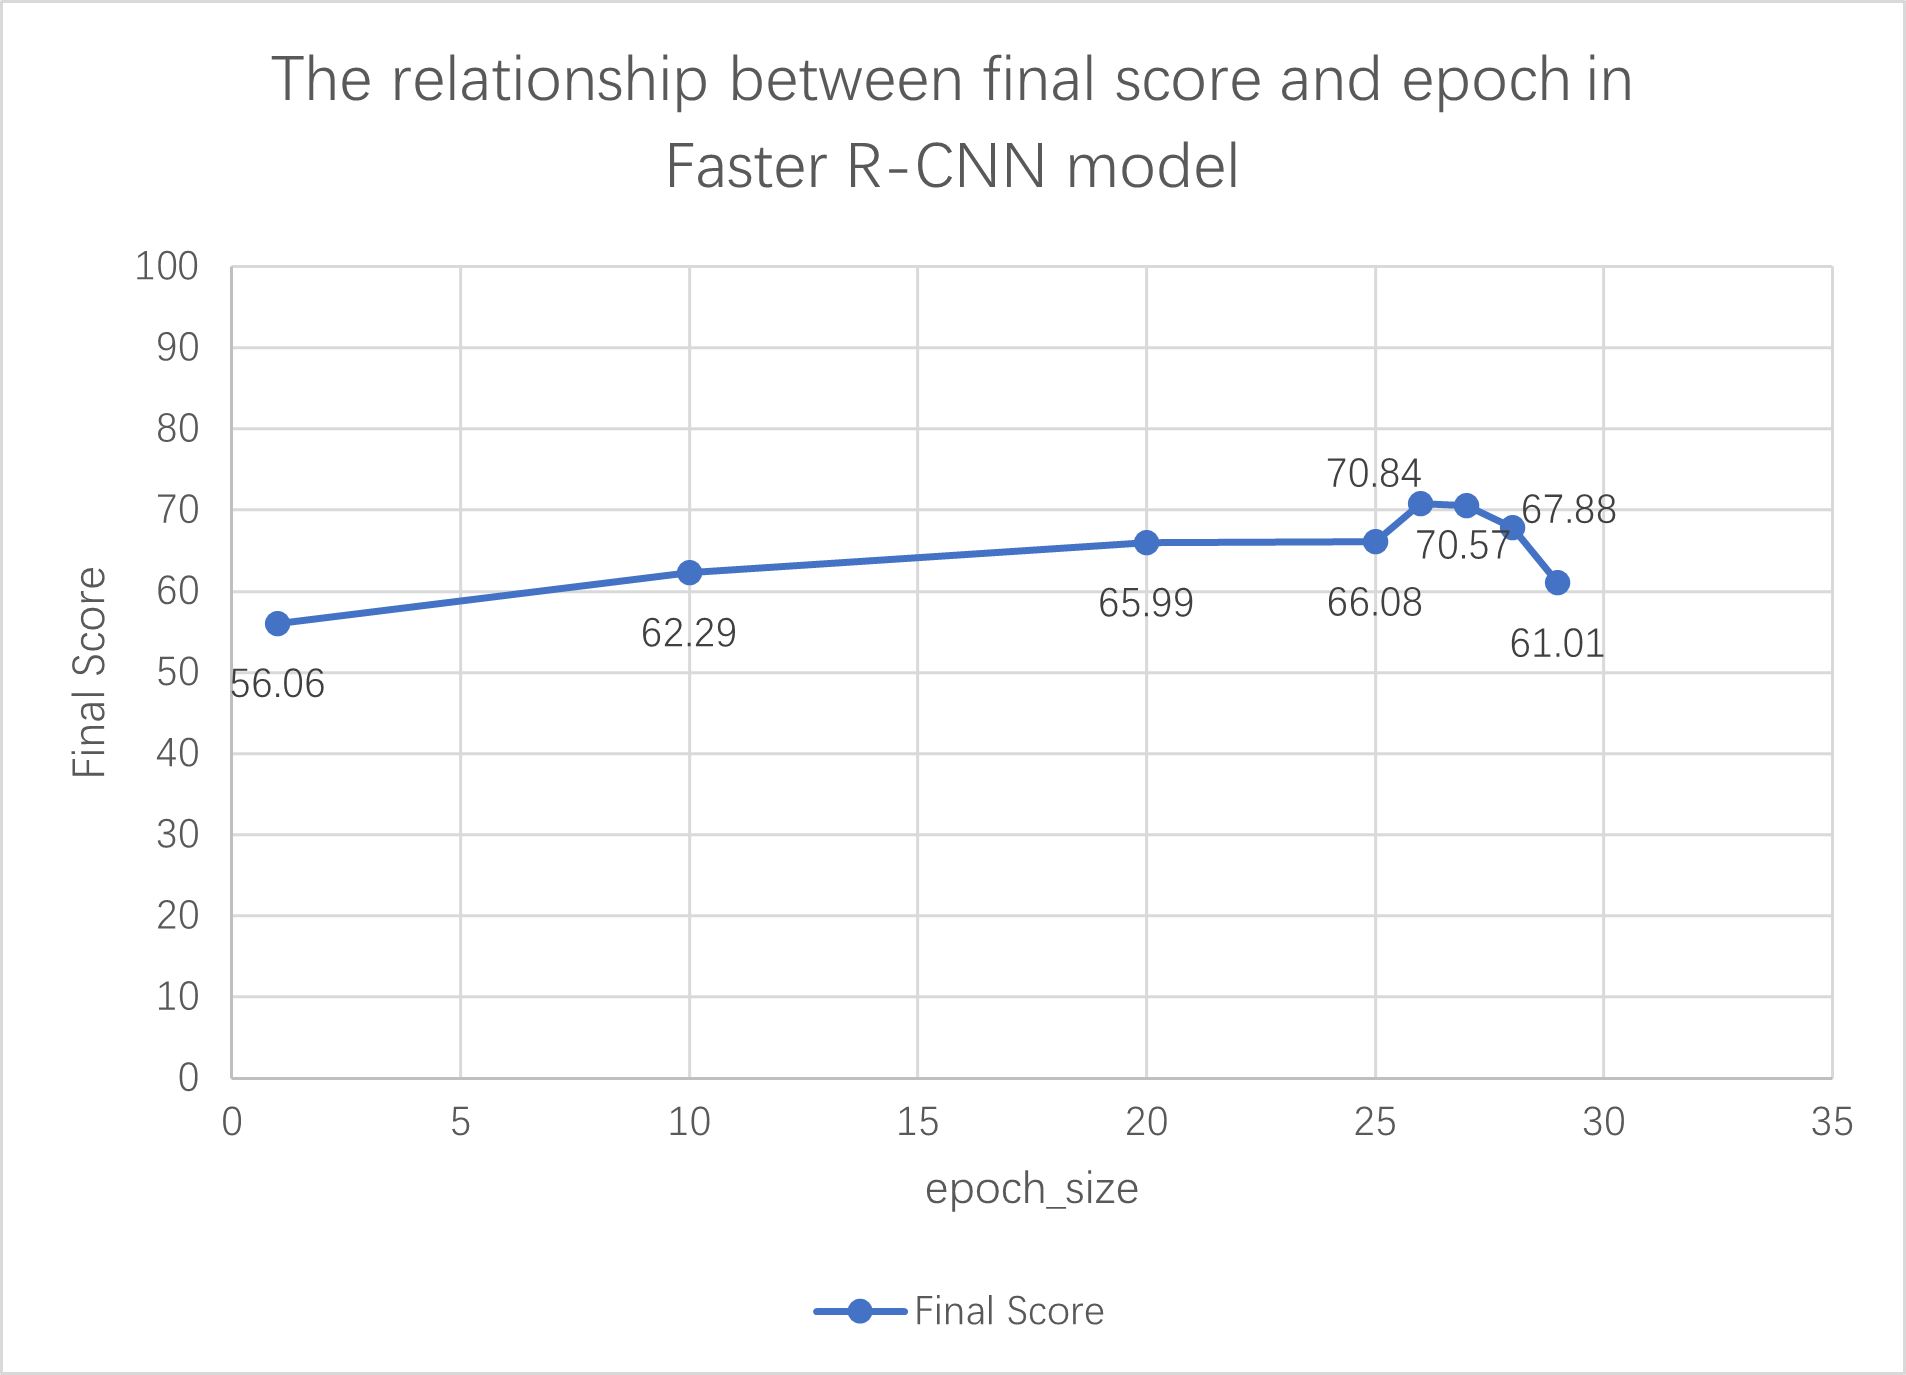
\includegraphics[width=0.8\linewidth]{./graphs/图片1.png}
  %\rule{0.9\linewidth}{0pt}
  %}

  \caption{Micro-F1 vs. Epochs for Faster-RCNN Model}
  \label{fig:faster-r-cnn}
\end{figure}

The initial Micro-F1 score of the Faster R-CNN model is 56.06. By increasing the epochs, we find that at epoch 26, the score reaches the maximum of 70.84. After further training, the score decreases, indicating that the model may have overfitted.

The Faster R-CNN model is easy to call and has a simple model definition. After 26 epochs, the model achieves the best score, but the training process is slow. Data augmentation significantly increases training time, and the results are not ideal. However, Faster R-CNN helps to understand the ResNet-50 network structure and the significance of hyperparameter tuning for model training.

\subsubsection{YOLOv8n}

Training with parameters $imgsz = 640,\ batch = 16$ and predicting with parameter $conf = 0.25$, we gradually increase the training epochs. The relationship between Micro-F1 score and epochs for the YOLOv8n model is shown in the line chart \cref{fig:yolov8n}.
\begin{figure}[t]
  \centering
  %\fbox{\rule{0pt}{2in}
  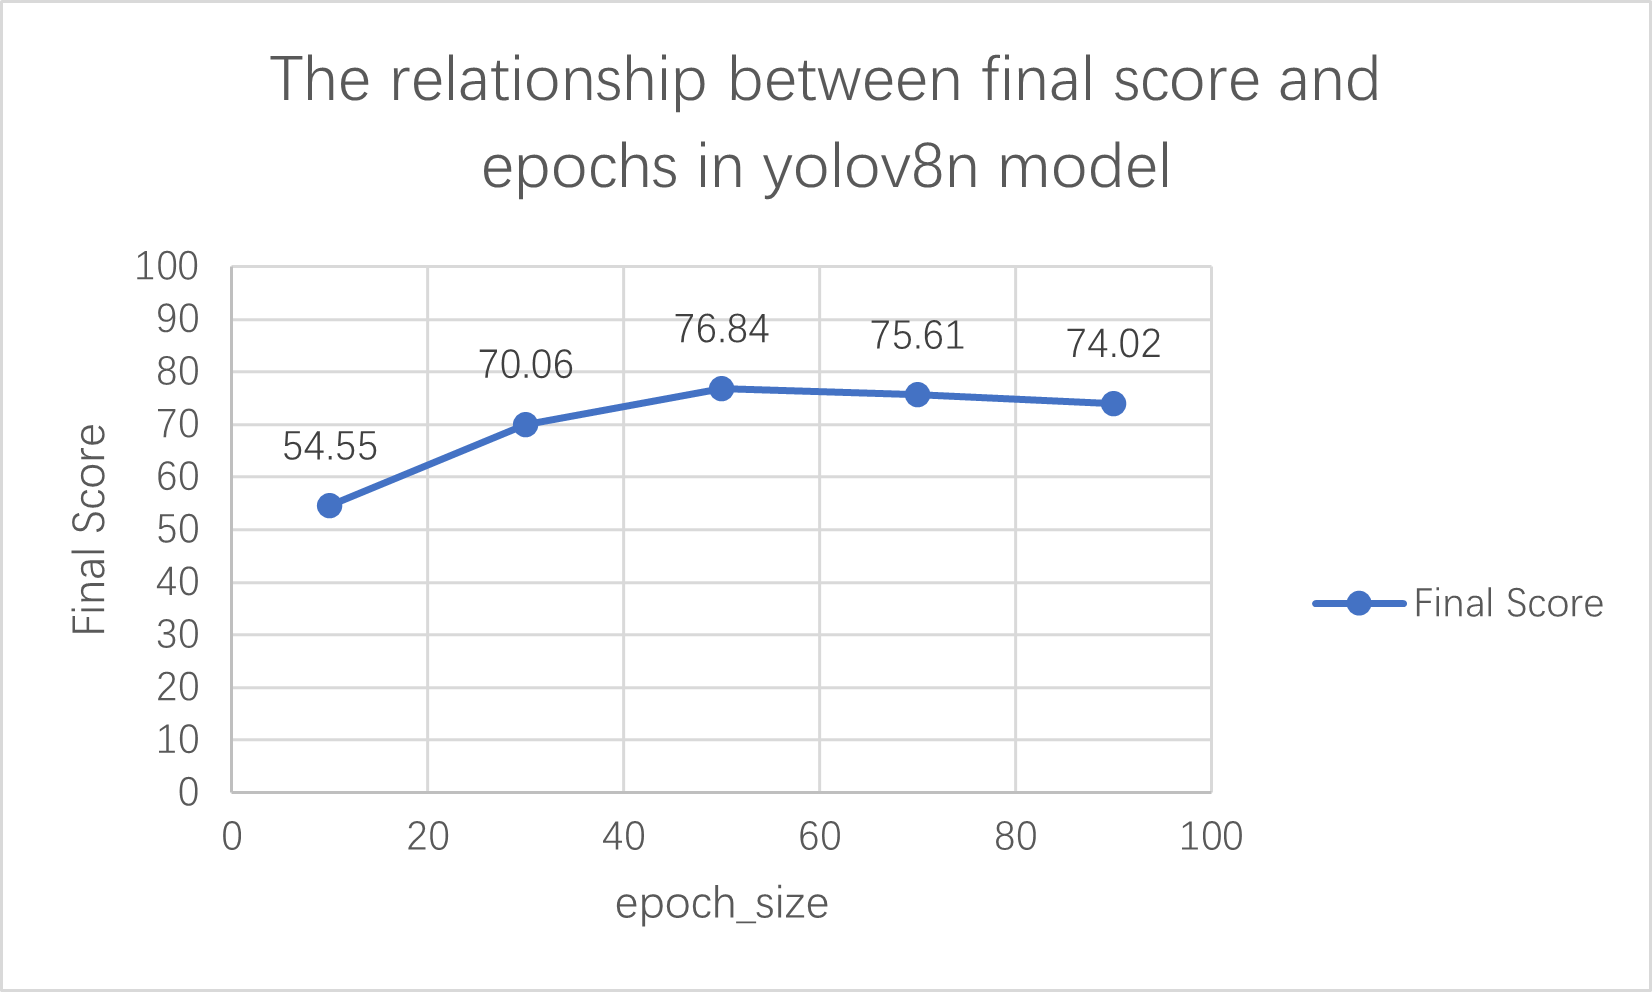
\includegraphics[width=0.8\linewidth]{./graphs/图片2.png}
  %\rule{0.9\linewidth}{0pt}
  %}

  \caption{Micro-F1 vs. Epochs for YOLOv8n Model}
  \label{fig:yolov8n}
\end{figure}

The number of training epochs has a significant effect on the score. After rough estimation, the model reaches its maximum score of 76.84 after around 50 epochs, surpassing Faster R-CNN. The YOLOv8n model trains much faster than Faster R-CNN, proving that the YOLO model is more flexible. Therefore, we consider using a larger model for training based on YOLO.

\subsubsection{YOLO Model Version Comparison}

Based on the YOLO model, we attempt to train with larger and newer models. Based on the baseline experiment results of YOLOv8n, we train YOLO11n and YOLO11m, and compare the results of epoch 50 and epoch 70 in a bar chart \cref{fig:yolo-compare}.
\begin{figure}[t]
  \centering
  %\fbox{\rule{0pt}{2in}
  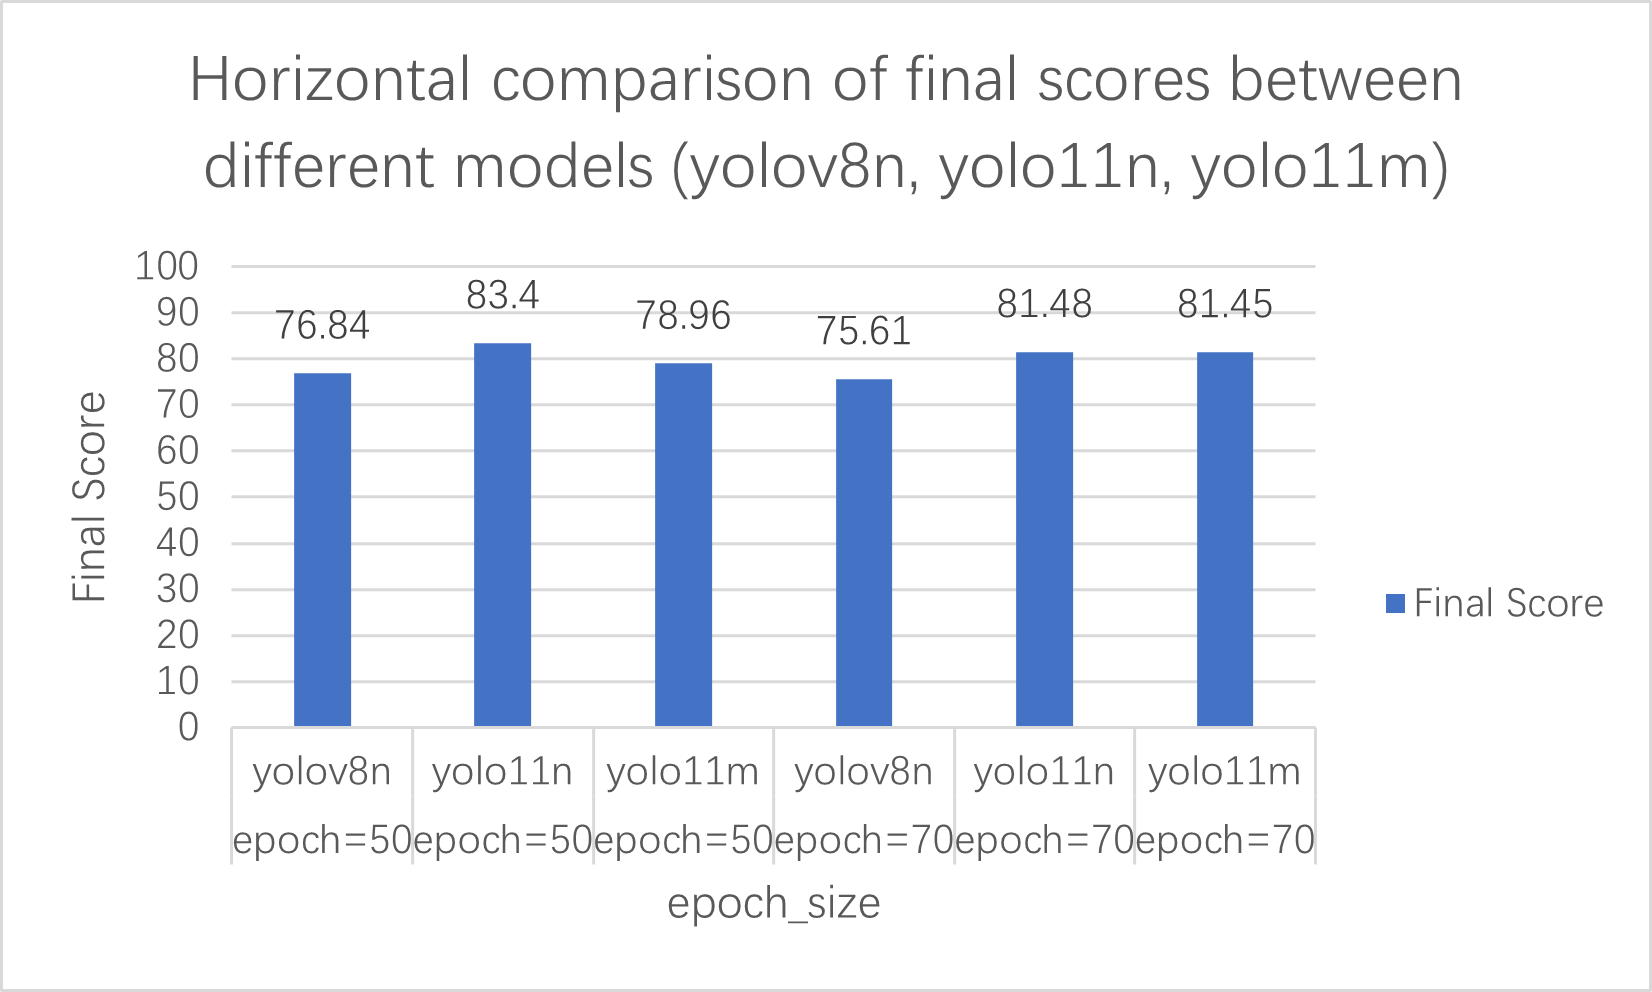
\includegraphics[width=0.8\linewidth]{./graphs/图片3.png}
  %\rule{0.9\linewidth}{0pt}
  %}

  \caption{Comparison of YOLOv8n, YOLO11n, and YOLO11m}
  \label{fig:yolo-compare}
\end{figure}

From the chart, it is clear that for the updated YOLO11 model, the accuracy is significantly higher than YOLOv8 when all other parameters are consistent. Although YOLO11m has a larger number of parameters, its accuracy is lower than YOLO11n in the chart. This suggests that the accuracy of the model is not only related to the number of parameters but also to other parameters (such as epoch and batch). When the epoch and batch are smaller, YOLO11m does not necessarily outperform YOLO11n. The subsequent \cref{subsec:create} section will carefully compare the effects of epoch and batch on YOLO11m, as the highest score is achieved by YOLO11m.

\subsection{Method Innovation}
\label{subsec:create}
\subsubsection{Innovation 1: Region Threshold Filtering}
To improve the model's detection performance on different images and provide multiple detection intervals, we modify the Faster R-CNN evaluation logic to set a confidence threshold for generating tampered regions. The code modification is shown in \cref{fig:faster-r-cnn-conf-code}.
\begin{figure}[t]
  \centering
  %\fbox{\rule{0pt}{2in}
  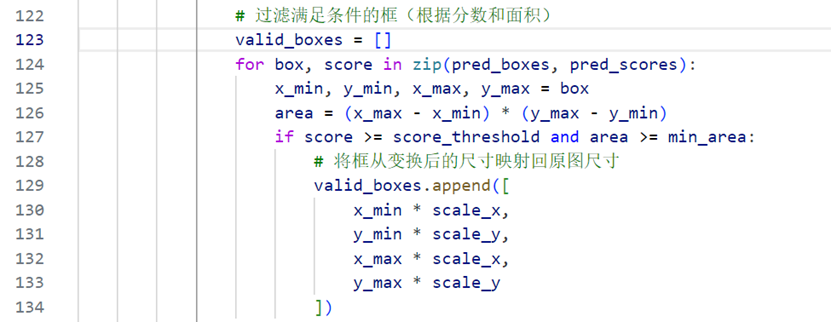
\includegraphics[width=0.8\linewidth]{./graphs/图片4.png}
  %\rule{0.9\linewidth}{0pt}
  %}

  \caption{Code Modification for Region Threshold Filtering}
  \label{fig:faster-r-cnn-conf-code}
\end{figure}

From the highest score point in \cref{fig:faster-r-cnn}, we compare the 26th and 27th epochs with and without region threshold filtering. The results are shown in the bar chart \cref{fig:faster-r-cnn-conf}.
\begin{figure}[t]
  \centering
  %\fbox{\rule{0pt}{2in}
  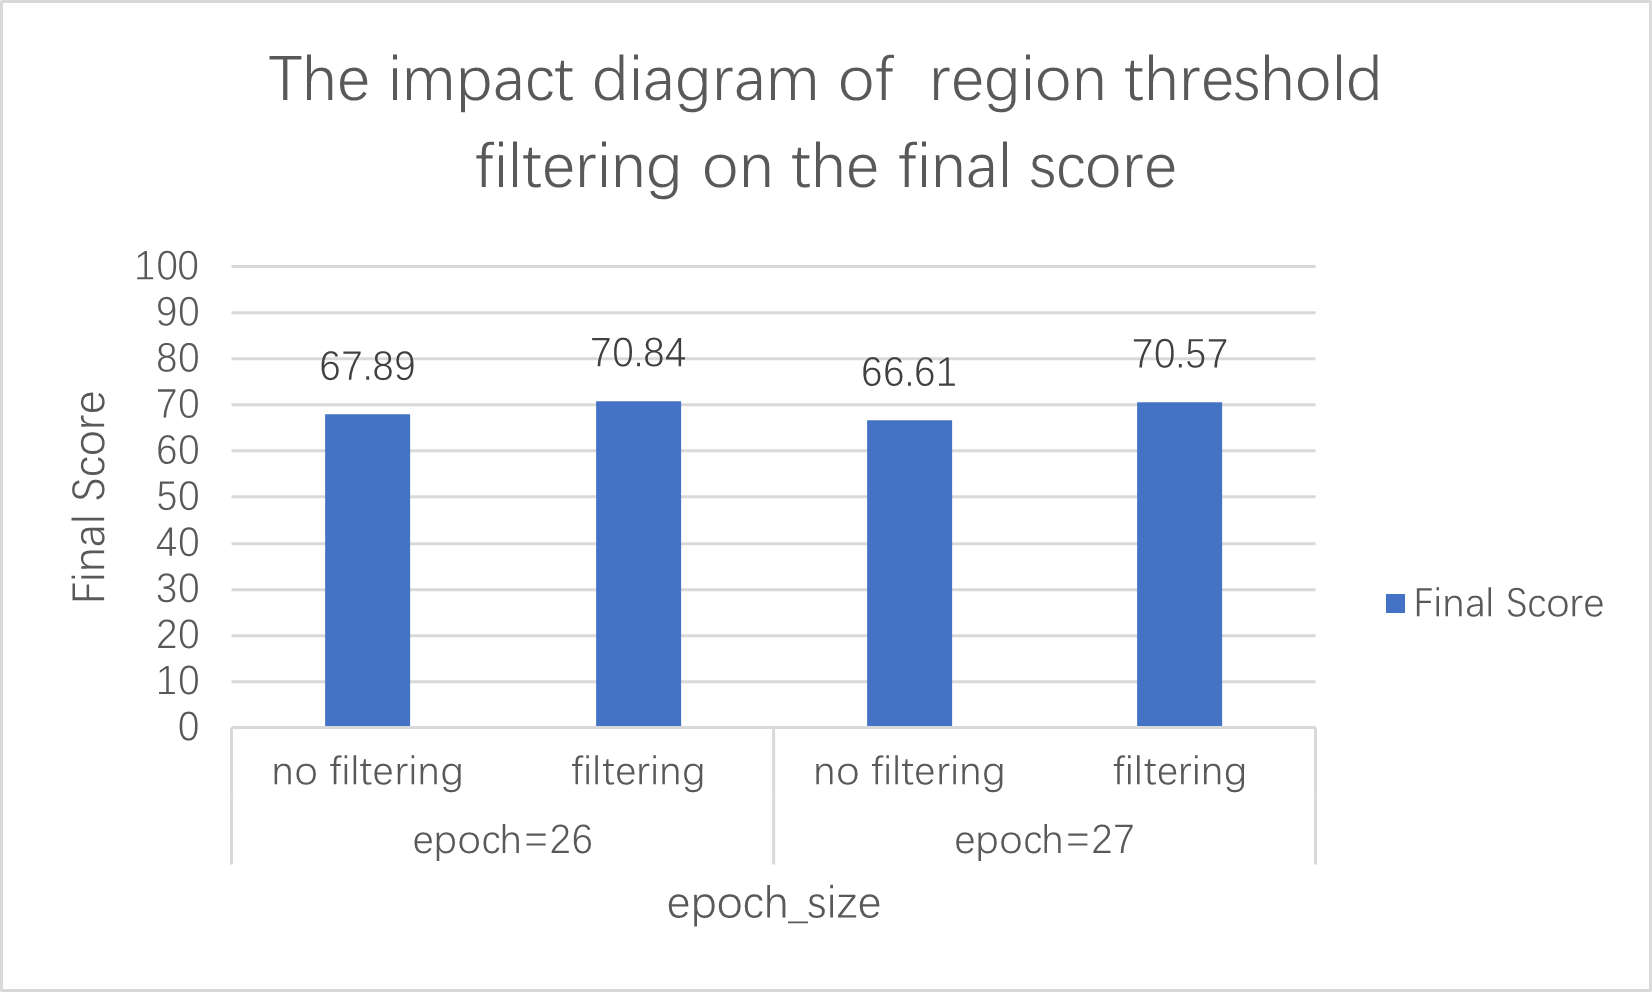
\includegraphics[width=0.8\linewidth]{./graphs/图片5.png}
  %\rule{0.9\linewidth}{0pt}
  %}

  \caption{Impact of Region Threshold Filtering in Faster R-CNN}
  \label{fig:faster-r-cnn-conf}
\end{figure}

From the chart, we can see that the score has significantly improved with the innovation of region threshold filtering, indicating that this method has a clear effect in this experiment.

\subsubsection{Innovation 2: Adjusting Training Parameters and Configuration Files}
In this section, we adjust the parameters for YOLO11m and gradually converge to the highest possible score for the YOLO model.

First, we modify the batch size and increase the number of training epochs. These two parameters have a significant impact on the prediction score. We train with batch sizes of 64 and 256 for 40, 60, and 80 epochs, and the results are shown in the bar chart \cref{fig:yolo-batchsize}.
\begin{figure}[t]
  \centering
  %\fbox{\rule{0pt}{2in}
  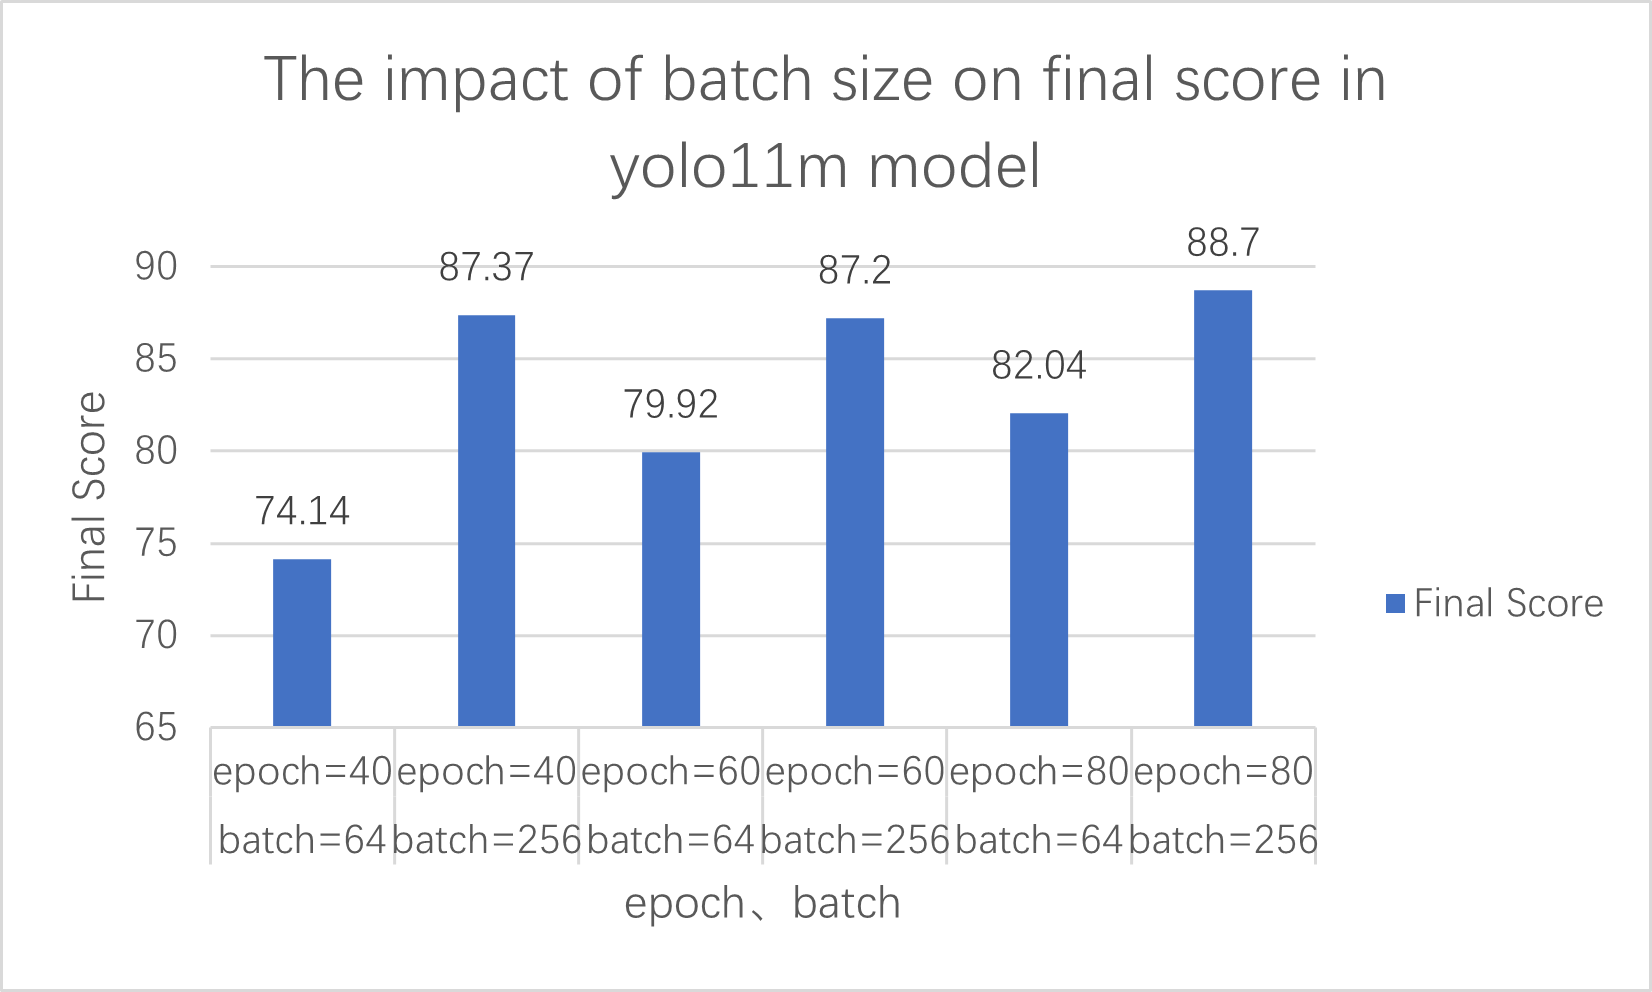
\includegraphics[width=0.8\linewidth]{./graphs/图片8.png}
  %\rule{0.9\linewidth}{0pt}
  %}

  \caption{Impact of Batch Size in YOLO11m Model}
  \label{fig:yolo-batchsize}
\end{figure}

From the chart, it is clear that increasing the batch size greatly helps the model's score, with a significant improvement. Increasing the batch size greatly enhances the model's ability under the same number of epochs.

With a batch size of 256, we increase the training epochs and obtain the line chart of prediction scores as epochs increase \cref{fig:yolo-epoch}.
\begin{figure}[t]
  \centering
  %\fbox{\rule{0pt}{2in}
  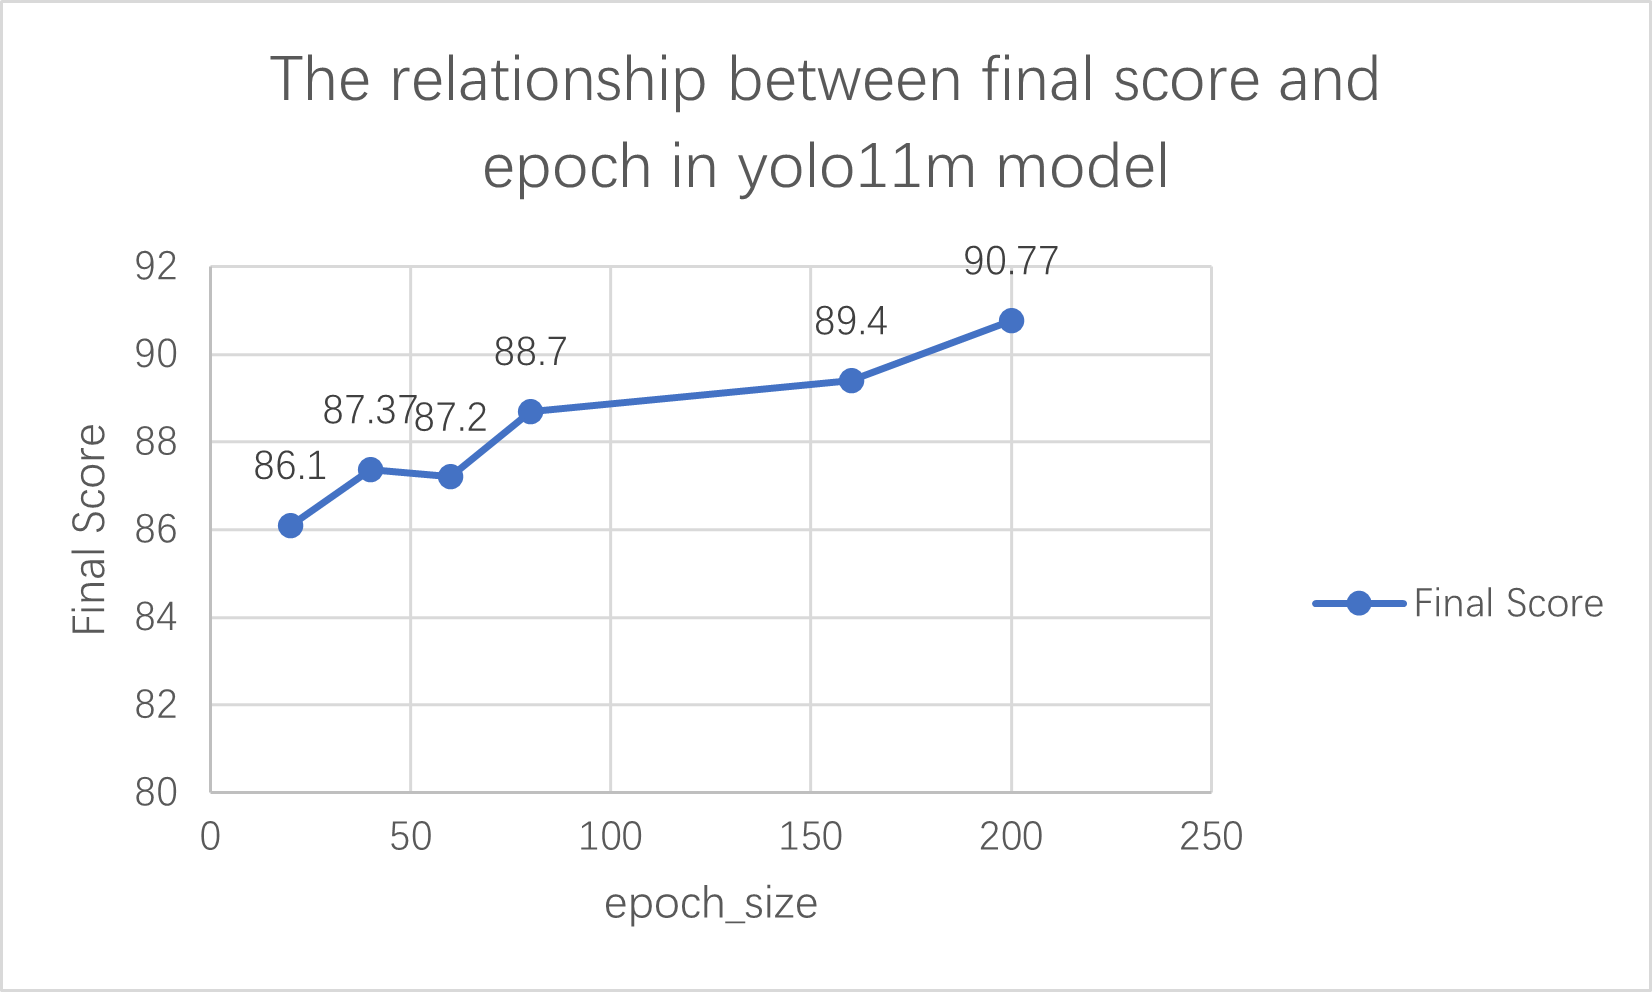
\includegraphics[width=0.8\linewidth]{./graphs/图片9.png}
  %\rule{0.9\linewidth}{0pt}
  %}

  \caption{Micro-F1 vs. Epochs for YOLO11m Model}
  \label{fig:yolo-epoch}
\end{figure}

From the chart, it can be seen that the YOLO11m model with batch = 256 is very powerful. While there are slight fluctuations during the increase in epochs, the overall trend is an upward one. At epoch = 200, the Micro-F1 score exceeds 90, which is a very high accuracy.

After adjusting the batch size and training epochs to make the model converge, we fine-tune the model by adjusting the confidence threshold ($conf$) and uniform image size ($image\_size$) to achieve a slight improvement in the score.

We set confidence thresholds to 0.3, 0.5, and 0.7, and compare the predicted results for epochs 50 and 200, as shown in the bar chart \cref{fig:yolo-conf}.

\begin{figure}[t]
  \centering
  %\fbox{\rule{0pt}{2in}
  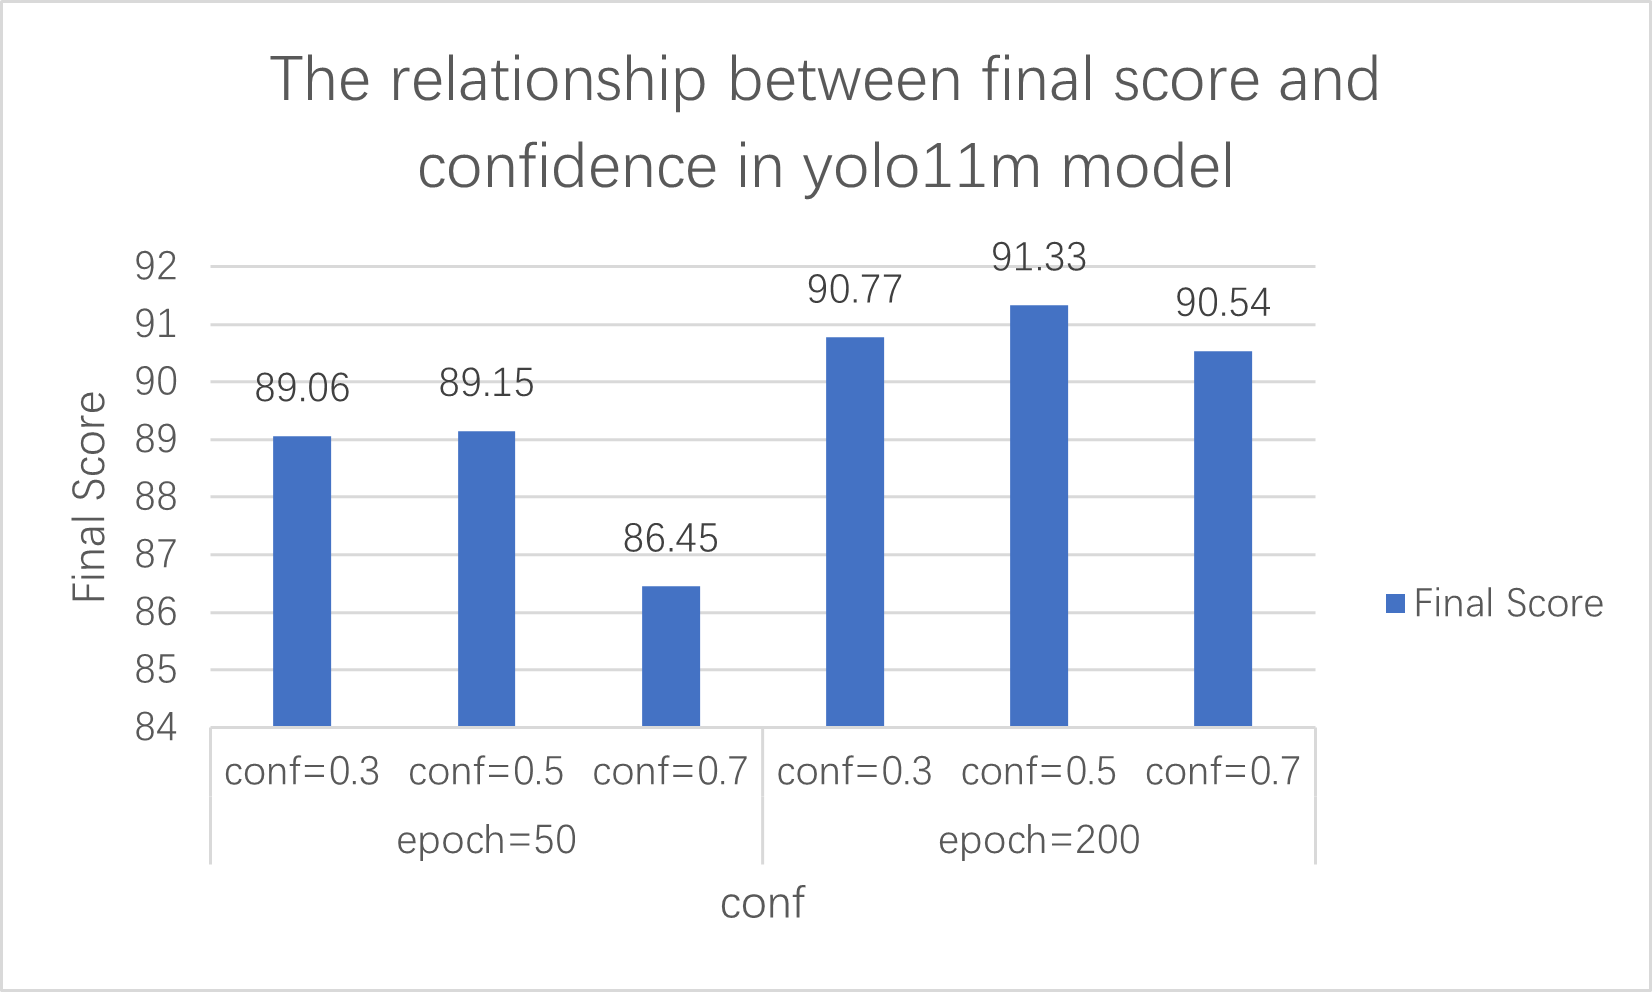
\includegraphics[width=0.8\linewidth]{./graphs/图片10.png}
  %\rule{0.9\linewidth}{0pt}
  %}

  \caption{Micro-F1 vs. Confidence Threshold in YOLO11m}
  \label{fig:yolo-conf}
\end{figure}

From the chart, it can be roughly seen that there is no definite pattern or conclusion between the confidence threshold and the model's score. Both too high and too low confidence thresholds lead to a decrease in model performance. The optimal confidence threshold varies after each training session. Therefore, confidence can only be used as a trial-and-error method to improve the model after finding the best one, and cannot directly determine the optimal confidence threshold for the model.

The results obtained from further testing, not shown in the figure, indicate that the model score reaches its optimal value of 93.68 when adjusting $conf = 0.2$.

Finally, we increase $image\_size$ to 800, which is the uniform size to which the images are scaled before training in the YOLO model. We compare the predicted results for epochs 150 and 200, as shown in the bar chart \cref{fig:yolo-size}.
\begin{figure}[t]
  \centering
  %\fbox{\rule{0pt}{2in}
  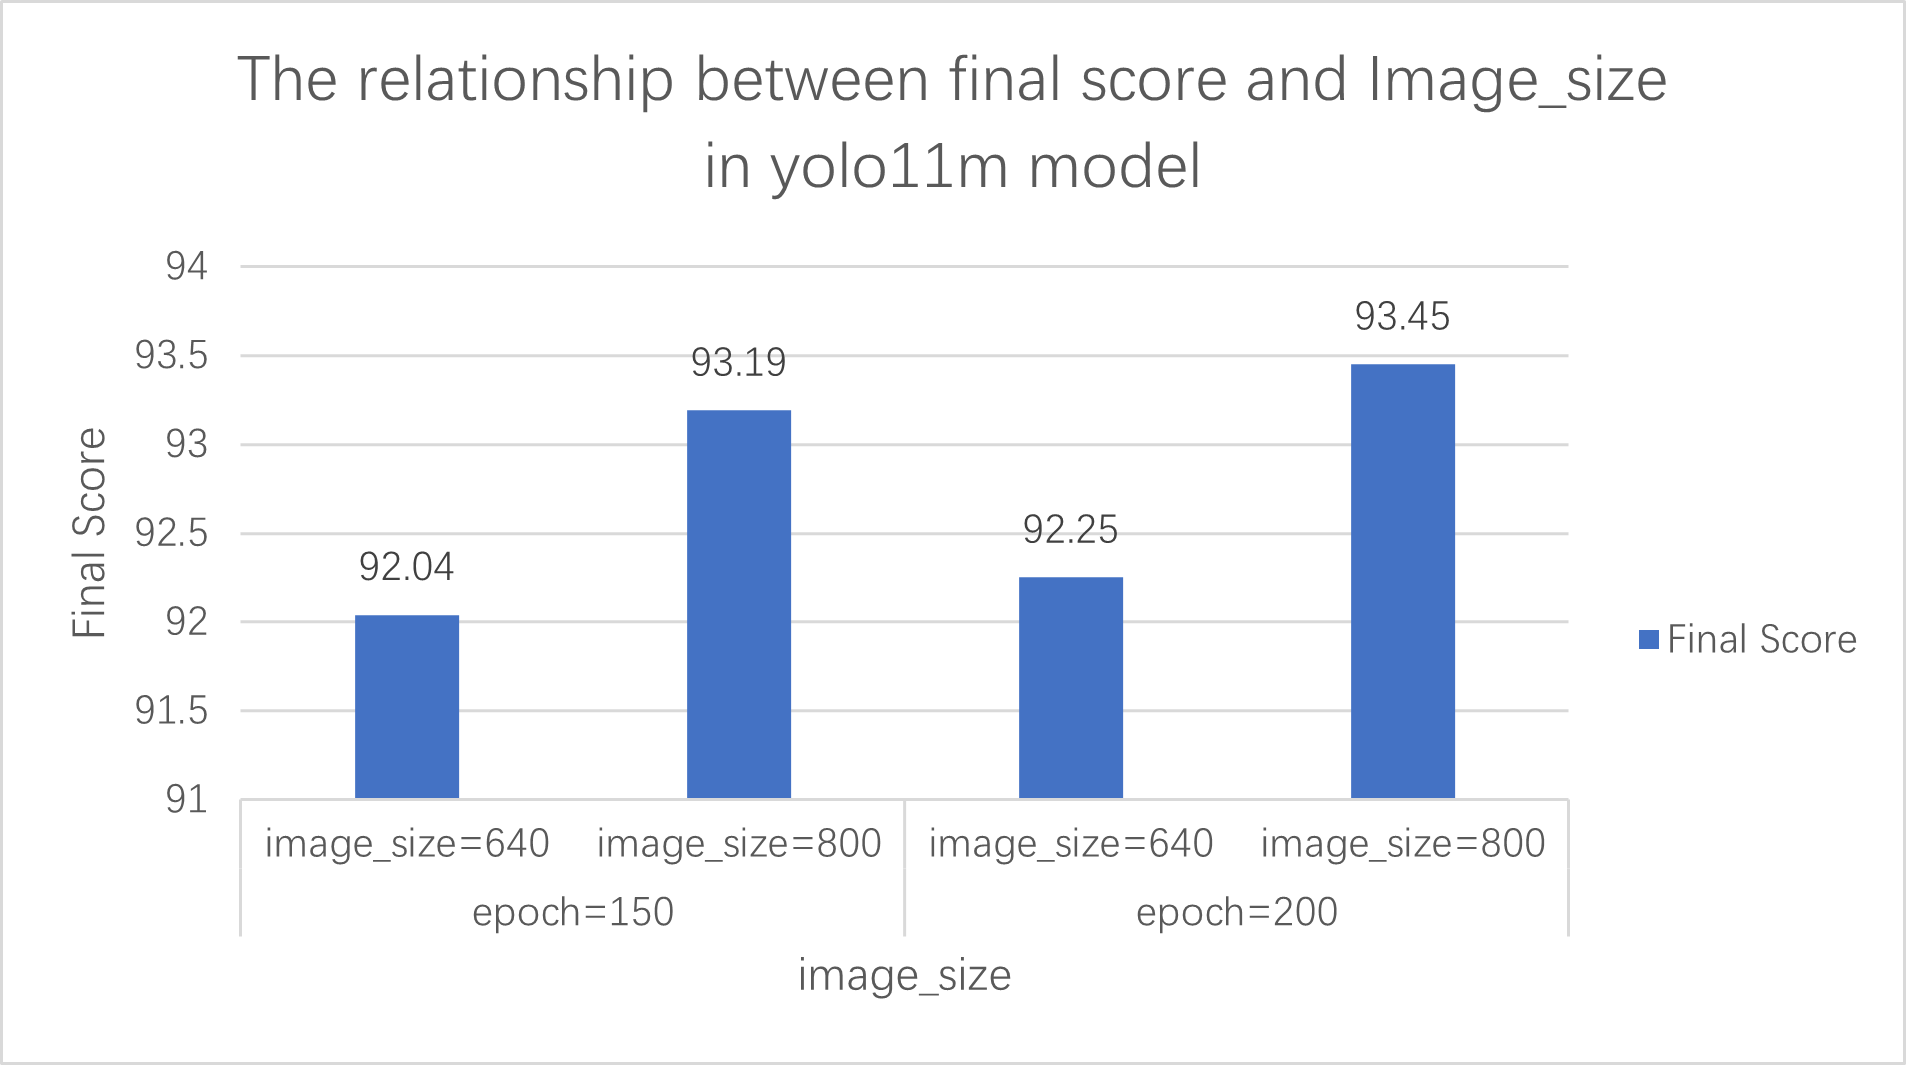
\includegraphics[width=0.8\linewidth]{./graphs/图片11.png}
  %\rule{0.9\linewidth}{0pt}
  %}

  \caption{Micro-F1 vs. Image Size in YOLO11m Model}
  \label{fig:yolo-size}
\end{figure}

Increasing the image size, though requiring more computing power, leads to better model performance because more information is preserved in the images.

\subsubsection{Innovation 3: Multi-scale Data Augmentation}

Due to data augmentation operations such as image flipping, the data volume can be expanded to make the network-trained model more accurate\cite{sym11101223}, which proved feasible for optimizing the scores. Therefore, we also tried multi-scale data augmentation.

To enhance the model's robustness to tampering at different scales, we introduce multi-scale image resizing during the training of YOLO11m. The data augmentation parameter configuration is shown in \cref{fig:yolo-data-code}.
\begin{figure}[t]
  \centering
  %\fbox{\rule{0pt}{2in}
  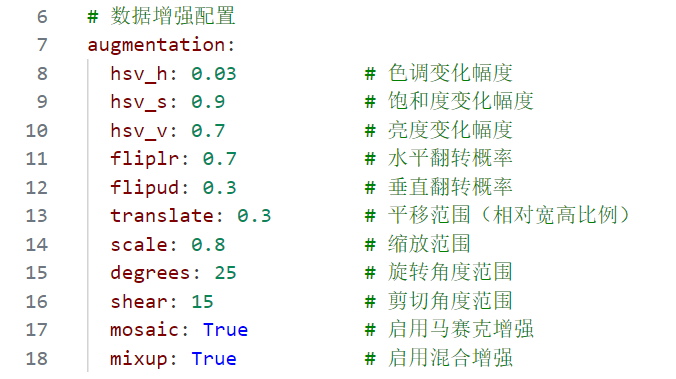
\includegraphics[width=0.8\linewidth]{./graphs/图片6.png}
  %\rule{0.9\linewidth}{0pt}
  %}

  \caption{Data Augmentation Parameter Configuration}
  \label{fig:yolo-data-code}
\end{figure}

We compare the prediction scores for epochs 150 and 200 with and without data augmentation, as shown in the bar chart \cref{fig:yolo-data}.
\begin{figure}[t]
  \centering
  %\fbox{\rule{0pt}{2in}
  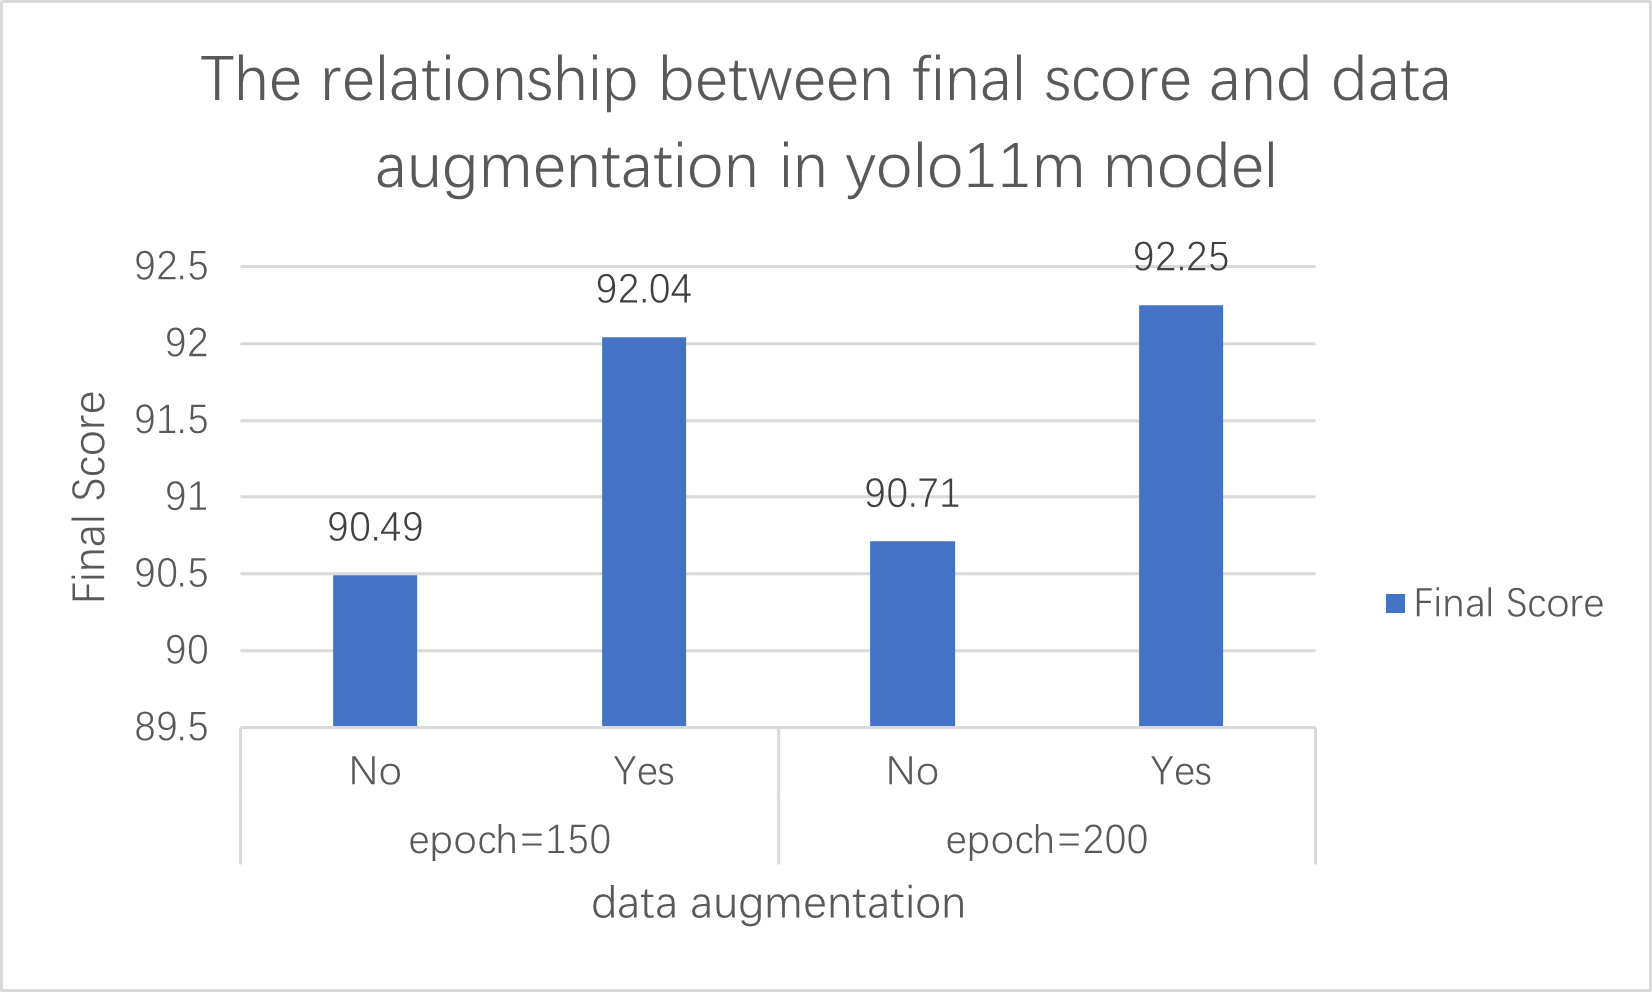
\includegraphics[width=0.8\linewidth]{./graphs/图片7.png}
  %\rule{0.9\linewidth}{0pt}
  %}

  \caption{Micro-F1 vs. Data Augmentation in YOLO11m Model}
  \label{fig:yolo-data}
\end{figure}

Before data augmentation, no matter what tuning method was applied, the highest score the model could achieve was 90.71. However, with data augmentation and the same training parameters, the model score reached 92.25, indicating that data augmentation has a significant effect on the YOLO model.

\subsection{Ablation Experiment Results}

Based on the comparisons in \cref{subsec:create} between Faster R-CNN models with and without region threshold filtering and parameter adjustments, and YOLO models with and without multi-scale data augmentation and parameter adjustments, we present the results in tables \cref{tab:xiaorong} and \cref{tab:xiaorong2} using Micro-F1 as the metric.

\begin{table}
  \centering
  \begin{tabular}{c|c|c|c}
    \toprule
    Model                         & Filter & Adjustment & Micro-F1 \\
    \midrule
    \multirow{3}{*}{Faster R-CNN} & No     & No         & 56.06    \\
                                  & No     & Yes        & 67.89    \\
                                  & Yes    & Yes        & 70.84    \\
    \bottomrule
  \end{tabular}
  \caption{Ablation Experiment Results Table for Faster R-CNN}
  \label{tab:xiaorong}
  \vspace{\baselineskip}
  \begin{tabular}{c|c|c|c}
    \toprule
    Model                 & Augmentation & Adjustment & Micro-F1 \\
    \midrule
    \multirow{3}{*}{YOLO} & No           & No         & 76.84    \\
                          & No           & Yes        & 90.71    \\
                          & Yes          & Yes        & 93.68   \\
    \bottomrule
  \end{tabular}
  \caption{Ablation Experiment Results Table for YOLO}
  \label{tab:xiaorong2}
\end{table}

Region threshold filtering significantly improved Faster R-CNN's performance on smaller tampered regions.

Multi-scale data augmentation improved YOLO11m's generalization ability across different tampering patterns.

Adjusting training parameters and configuration files also resulted in an increase in score over the model's baseline.

\section{Experimental Results and Analysis}
\label{sec:result}
%-------------------------------------------------------------------------

\subsection{Best Results}

\noindent
The highest Micro-F1 score achieved so far is 93.68. This score is shown in the competition website as \cref{fig:final-score}.

\begin{figure*}
    \centering
    \begin{subfigure}{0.75\linewidth}
        %\%fbox{\rule{0pt}{2in} \rule{.9\linewidth}{0pt}}
        
\includegraphics[width=\linewidth]{./graphs/图片14.png}
        %\caption{An example of a subfigure.}
        \label{fig:final-score1}
    \end{subfigure}
    %\hfill
    \begin{subfigure}{0.2\linewidth}
        %\fbox{\rule{0pt}{2in} \rule{.9\linewidth}{0pt}}
        
\includegraphics[width=\linewidth]{./graphs/图片15.png}
        %\caption{Another example of a subfigure.}
        \label{fig:final-score2}
    \end{subfigure}
    \caption{Screenshot of Final Score in the Competition Website}
    \label{fig:final-score}
\end{figure*}

\noindent
The experimental parameters that yielded the highest score are as follows:

\noindent
\textbf{Model:} YOLO11m

\noindent
\textbf{Number of Training Epochs:} 200

\noindent
\textbf{Unified Image Size during Training:} 800$\times$800 pixels

\noindent
\textbf{Batch:} 256

\noindent
\textbf{Prediction Confidence:} 0.2

\subsection{Result Analysis}

Based on the analysis and comparison of the performance of each model during the experiments in \cref{sec:steps}, the following conclusions can be made:

\subsubsection{Performance Analysis of Faster R-CNN}
Faster R-CNN is a precision-first two-stage object detection model that demonstrated high reliability and accuracy in this experiment, particularly in locating and classifying small targets. The experiment showed the following:

The baseline Micro-F1 score was 56.06, with limited performance when no region threshold filtering or parameter tuning was applied.

After adding region threshold filtering, the Micro-F1 score improved to 70.84, significantly enhancing the model's ability to detect small tampered regions.

However, Faster R-CNN has a slower training speed and higher computational resource demands, especially when data augmentation is used, leading to significantly increased training time. While the performance is acceptable, it is not suitable for efficient large-scale detection solutions.

\subsubsection{Performance Analysis of the YOLO Model}
YOLO models are known for their fast detection performance and strong generalization capability, particularly in small object detection and real-time applications. In the experiment:

YOLOv8n achieved a baseline Micro-F1 score of 76.84, significantly higher than Faster R-CNN.

Although YOLO11m has a larger number of parameters, it performed optimally with sufficient training (such as increasing epochs and batch size), with the Micro-F1 score exceeding 93. This indicates that YOLO models have strong adaptability to large-scale training.

\subsubsection{Horizontal Comparison Between Models}

Faster R-CNN is suitable for detection tasks that require high precision, but it has significant disadvantages in training speed and scalability.

YOLO series models, especially YOLO11m, strike a better balance between speed and accuracy, outperforming both Faster R-CNN and YOLOv8.

\subsubsection{Effectiveness of Innovative Methods}

\textbf{Region Threshold Filtering:} Introducing region threshold filtering for Faster R-CNN significantly improved the model's ability to recognize small targets, which was a key method for enhancing its performance.

\textbf{Training Parameter Adjustment:} For YOLO11m, adjusting the batch size (from 64 to 256), increasing the number of training epochs (up to 200) and increasing the $image\_size$ (up to 800) gradually improved the Micro-F1 score, indicating that larger batch training aids in enhancing model performance.

\textbf{Multi-Scale Data Augmentation:} By incorporating multi-scale data augmentation with different scaling sizes, the robustness of the model in detecting various tampering patterns was significantly improved, with the Micro-F1 score of YOLO11m rising from 90.71 to 92.25. This confirmed the importance of multi-scale multi-scale data augmentation in improving the model's generalization ability.

In summary, this experiment validated the efficiency and strong performance of YOLO11m, and the innovative methods (such as region threshold filtering and multi-scale data augmentation) significantly improved the model's Micro-F1 score, ultimately reaching 93.68. This demonstrates that through careful parameter tuning and the introduction of innovative techniques, it is possible to effectively optimize model performance and improve the accuracy of document tampering detection.

\subsection{Future Work}

Explore hybrid architectures combining the precision of Faster R-CNN and the speed of YOLO.

Experiment with larger models (\eg SAM) and evaluate their performance in more complex scenarios.

\subsection{About the Code}

A complete codebase and configuration files are provided to ensure result reproducibility.

The scripts have been optimized to accommodate various hardware environments. When using the code, the user needs to change its relative path.

The purposes of the code files in the "Codes" folder are as follows:

YOLO/eval\_yolo.py generates json file according to the YOLO model.

YOLO/transform.py turns the origin data into the right format for YOLO model.

YOLO/train.py is the YOLO training code.

YOLO/split.py divides the training data into training set and validation set randomly.

YOLO/coco.yaml is the configuration file for YOLO.

Faster R-CNN/Faster-RCNN-eval.py generates json file according to the Faster R-CNN model.

Faster R-CNN/Faster-RCNN-train.py is the Faster R-CNN training code.
\section{Team Information}
\label{sec:group}

\subsection{Team Members Information}

郑光铭 22302010014

陈柏滔 22302010008

黄宸一 22302010011

\subsection{Team Name}

专业课和我作队

\subsection{Contribution Distribution}

郑光铭: 40\%

陈柏滔: 40\%

黄宸一: 20\%

\nocite{sym11101223}
\nocite{SANDHYA2024301663}
\nocite{18512}
\nocite{LiuHaoyue2021RGBN}
\nocite{article}
\nocite{8977568}


{
    \small
    \bibliographystyle{ieeenat_fullname}
    \bibliography{main}
}

% WARNING: do not forget to delete the supplementary pages from your submission 
% \clearpage
\setcounter{page}{1}
\maketitlesupplementary


\section{Rationale}
\label{sec:rationale}
% 
Having the supplementary compiled together with the main paper means that:
% 
\begin{itemize}
\item The supplementary can back-reference sections of the main paper, for example, we can refer to \cref{sec:intro};
\item The main paper can forward reference sub-sections within the supplementary explicitly (e.g. referring to a particular experiment); 
\item When submitted to arXiv, the supplementary will already included at the end of the paper.
\end{itemize}
% 
To split the supplementary pages from the main paper, you can use \href{https://support.apple.com/en-ca/guide/preview/prvw11793/mac#:~:text=Delete%20a%20page%20from%20a,or%20choose%20Edit%20%3E%20Delete).}{Preview (on macOS)}, \href{https://www.adobe.com/acrobat/how-to/delete-pages-from-pdf.html#:~:text=Choose%20%E2%80%9CTools%E2%80%9D%20%3E%20%E2%80%9COrganize,or%20pages%20from%20the%20file.}{Adobe Acrobat} (on all OSs), as well as \href{https://superuser.com/questions/517986/is-it-possible-to-delete-some-pages-of-a-pdf-document}{command line tools}.

\end{document}
